
\providecommand{\Cat}{\mathcal{C}at}

\section{\trAdjunction{}与\trMate}\label{sec:adjunctions-and-mates}

正如第 2 章中所讨论的，任何 2-\trCategory{}都有一个内部定义的\trAdjunction{}概念，
由下列数据构成：
\begin{itemize}
\item 一对对象 $a$ 与 $b$；
\item 一对 1-\trCell{} $u\colon a\to b$ 与 $f\colon b\to a$；以及
\item 一对 2-\trCell{} $\eta\colon 1_{b}\Rightarrow uf$ 与
  $\epsilon\colon fu\Rightarrow 1_{a}$，分别称为\textbf{\trUnit}与%
\textbf{\trCounit}，
\end{itemize}
使得\trTriangleEqualities{}成立：
\begin{center}
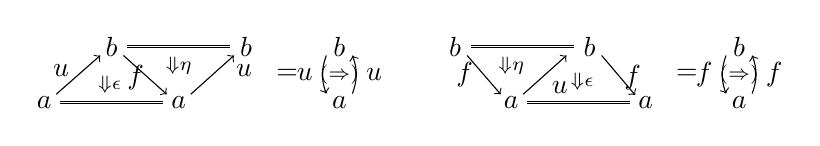
\begin{tikzpicture}[x=1.35em,y=1.35em]
  \node (A1) at (0,0) {$a$};
  \node (A2) at (3.6,0) {$a$};
  \node (B1) at (1.8,1.5) {$b$};
  \node (B2) at (5.4,1.5) {$b$};
  \draw[double] (0.42,0) -- (3.18,0);
  \draw[double] (2.22,1.5) -- (4.98,1.5);
  \draw[->] (0.32,0.22) -- (1.5,1.26);
  \node at (0.45,0.85) {$u$};
  \draw[->] (2.12,1.26) -- (3.28,0.22);
  \node at (2.45,0.68) {$f$};
  \draw[->] (3.92,0.22) -- (5.08,1.26);
  \node at (5.35,0.85) {$u$};
  \node at (1.75,0.48) {$\scriptstyle\Downarrow\epsilon$};
  \node at (3.6,1.0) {$\scriptstyle\Downarrow\eta$};
  \node at (6.5,0.75) {$=$};
  \node (Bs) at (7.9,1.5) {$b$};
  \node (As) at (7.9,0) {$a$};
  \draw[->] (7.55,1.26) to[bend right=20] node[left]{$u$} (7.55,0.24);
  \draw[->] (8.25,0.24) to[bend right=20] node[right]{$u$} (8.25,1.26);
  \node at (7.9,0.75) {$\scriptstyle(\Rightarrow)$};
  \node (B3) at (11.0,1.5) {$b$};
  \node (B4) at (14.6,1.5) {$b$};
  \node (A3) at (12.5,0) {$a$};
  \node (A4) at (16.1,0) {$a$};
  \draw[double] (11.42,1.5) -- (14.18,1.5);
  \draw[double] (12.92,0) -- (15.68,0);
  \draw[->] (11.32,1.26) -- (12.22,0.22);
  \node at (11.25,0.75) {$f$};
  \draw[->] (12.82,0.22) -- (13.98,1.26);
  \node at (13.8,0.4) {$u$};
  \draw[->] (14.92,1.26) -- (15.82,0.2);
  \node at (15.75,0.68) {$f$};
  \node at (12.5,1.0) {$\scriptstyle\Downarrow\eta$};
  \node at (14.4,0.55) {$\scriptstyle\Downarrow\epsilon$};
  \node at (17.2,0.75) {$=$};
  \node (Bt) at (18.6,1.5) {$b$};
  \node (At) at (18.6,0) {$a$};
  \draw[->] (18.25,1.26) to[bend right=20] node[left]{$f$} (18.25,0.24);
  \draw[->] (18.95,0.24) to[bend right=20] node[right]{$f$} (18.95,1.26);
  \node at (18.6,0.75) {$\scriptstyle(\Rightarrow)$};
\end{tikzpicture}
\end{center}

1-\trCell{} $f$ 称为\textbf{\trLeftAdjoint}，$u$ 称为\textbf{\trRightAdjoint}；
这一关系在行文中以 $f\dashv u$ 记之，在展示图中则画成如下之图：
\begin{rveq}\label{eq:adjunction-diagram}
\mbox{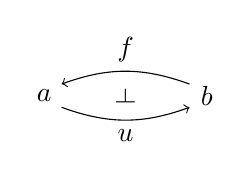
\begin{tikzpicture}[x=1.4em,y=1.4em]
  \node (a) at (0,0) {$a$};
  \node (b) at (4.2,0) {$b$};
  \draw[->] (3.75,0.3) to[bend right=20] node[above]{$f$} (0.45,0.3);
  \node[rotate=-90] at (2.1,0) {$\dashv$};
  \draw[->] (0.45,-0.3) to[bend right=20] node[below]{$u$} (3.75,-0.3);
\end{tikzpicture}}
\end{rveq}

关于\trAdjunction{}的基础 2-\trCategory{}论在 §2.1 中得到发展，其诸结果经
特殊化便可证明关于\trInfinityCategory{}之间\trAdjunction{}的定理。在此，我们沿一个
互补的方向拓广该理论——发展\emph{\trMate}（mates）的演算，它推广了人们更为熟悉的%
\trAdjunction{}转置。

当出现如 \eqref{eq:adjunction-diagram} 所示的\trAdjunction{}时，某些以 $a$ 为
余定义域的 2-\trCell{}可「转置」为以 $b$ 为余定义域的 2-\trCell{}；反对偶地，
某些以 $a$ 为定义域的 2-\trCell{}可「转置」为以 $b$ 为定义域的 2-\trCell{}：
对任何 1-\trCell{} $w\xrightarrow{x}b$、$w\xrightarrow{y}a$、$b\xrightarrow{h}z$
与 $a\xrightarrow{k}z$，
\begin{rveq}\label{eq:transposes}
fx\;\overset{\alpha}{\Longrightarrow}\;y\;\;\rightsquigarrow\;\;
x\;\overset{\beta}{\Longrightarrow}\;uy
\qquad\qquad
hu\;\overset{\gamma}{\Longrightarrow}\;k\;\;\rightsquigarrow\;\;
h\;\overset{\delta}{\Longrightarrow}\;kf
\end{rveq}
这两种转置操作都容许一个归于 Kelly 与 Street \cite{bib70} 的共同推广，称为
「\trMate」（mates correspondence），它描述由一对\trAdjunction{}所诱导的诸%
2-\trCell{}之间的一种对偶性。

\begin{definition}[\trMate]\label{def:mates}
给定任意一对\trAdjunction{}与\trFunctor
\begin{center}
\begin{tikzpicture}[x=1.9em,y=1.5em]
  \node (b)  at (0,1.5)  {$b$};
  \node (bp) at (3.6,1.5) {$b'$};
  \node (a)  at (0,0)    {$a$};
  \node (ap) at (3.6,0)  {$a'$};
  \draw[->] (0.5,1.5) -- node[above]{$\scriptstyle k$} (3.1,1.5);
  \draw[->] (0.5,0)   -- node[below]{$\scriptstyle h$} (3.1,0);
  \node[left] at (-0.25,0.75) {$f\dashv u$};
  \node[right] at (3.85,0.75) {$f'\dashv u'$};
\end{tikzpicture}
\end{center}
则在如下左侧的 2-\trCell{}与如下右侧的 2-\trCell{}之间存在一个双射
\begin{rveq}\label{eq:mates-bijection}
\mbox{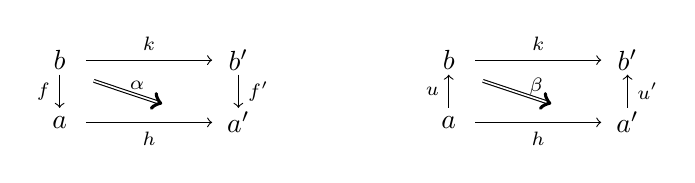
\begin{tikzpicture}[x=1.9em,y=1.5em]
  \node (lb)  at (0,1.5)  {$b$};
  \node (lbp) at (3.4,1.5) {$b'$};
  \node (la)  at (0,0)    {$a$};
  \node (lap) at (3.4,0)  {$a'$};
  \draw[->] (0.5,1.5) -- node[above]{$\scriptstyle k$} (2.9,1.5);
  \draw[->] (0.5,0)   -- node[below]{$\scriptstyle h$} (2.9,0);
  \draw[->] (0,1.15)  -- node[left]{$\scriptstyle f$} (0,0.35);
  \draw[->] (3.4,1.15) -- node[right]{$\scriptstyle f'$} (3.4,0.35);
  \draw[->,double] (0.65,1.0) -- (1.95,0.45);
  \node[right] at (1.15,0.9) {$\scriptstyle\alpha$};
  \node at (5.4,0.75) {$\rightsquigarrow$};
  \node (rb)  at (7.4,1.5)  {$b$};
  \node (rbp) at (10.8,1.5) {$b'$};
  \node (ra)  at (7.4,0)    {$a$};
  \node (rap) at (10.8,0)   {$a'$};
  \draw[->] (7.9,1.5) -- node[above]{$\scriptstyle k$} (10.3,1.5);
  \draw[->] (7.9,0)   -- node[below]{$\scriptstyle h$} (10.3,0);
  \draw[->] (7.4,0.35)  -- node[left]{$\scriptstyle u$} (7.4,1.15);
  \draw[->] (10.8,0.35) -- node[right]{$\scriptstyle u'$} (10.8,1.15);
  \draw[->,double] (8.05,1.0) -- (9.35,0.45);
  \node[right] at (8.75,0.85) {$\scriptstyle\beta$};
\end{tikzpicture}}
\end{rveq}
其通过将诸\trAdjunction{}的\trUnit{}与\trCounit{}作粘贴而实现：
\begin{center}
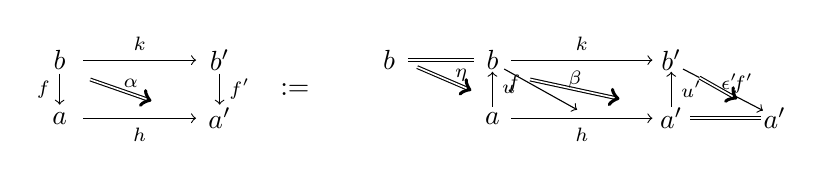
\begin{tikzpicture}[x=1.7em,y=1.4em]
  \node (ab)  at (0,1.5)  {$b$};
  \node (abp) at (3.4,1.5) {$b'$};
  \node (aa)  at (0,0)    {$a$};
  \node (aap) at (3.4,0)  {$a'$};
  \draw[->] (0.5,1.5) -- node[above]{$\scriptstyle k$} (2.9,1.5);
  \draw[->] (0.5,0)   -- node[below]{$\scriptstyle h$} (2.9,0);
  \draw[->] (0,1.15)  -- node[left]{$\scriptstyle f$} (0,0.35);
  \draw[->] (3.4,1.15) -- node[right]{$\scriptstyle f'$} (3.4,0.35);
  \draw[->,double] (0.65,1.0) -- (1.95,0.45);
  \node[right] at (1.15,0.9) {$\scriptstyle\alpha$};
  \node at (5.0,0.75) {$:=$};
  \node (pb)  at (7.0,1.5) {$b$};
  \node (pbm) at (9.2,1.5) {$b$};
  \node (pbp) at (13.0,1.5) {$b'$};
  \node (pa)  at (9.2,0) {$a$};
  \node (pam) at (13.0,0) {$a'$};
  \node (pap) at (15.2,0) {$a'$};
  \draw[double] (7.4,1.5) -- (8.8,1.5);
  \draw[->] (9.6,1.5) -- node[above]{$\scriptstyle k$} (12.6,1.5);
  \draw[->] (9.45,1.27) -- (11.0,0.22);
  \node[left] at (10.0,0.9) {$\scriptstyle f$};
  \draw[->,double] (7.6,1.32) -- (8.75,0.72);
  \node[right] at (8.2,1.1) {$\scriptstyle\eta$};
  \draw[->] (9.2,0.3) -- node[right]{$\scriptstyle u$} (9.2,1.2);
  \draw[->] (9.6,0) -- node[below]{$\scriptstyle h$} (12.6,0);
  \draw[->,double] (10.0,1.0) -- (11.9,0.5);
  \node[right] at (10.6,1.0) {$\scriptstyle\beta$};
  \draw[->] (13.0,0.3) -- node[right]{$\scriptstyle u'$} (13.0,1.2);
  \draw[->] (13.25,1.27) -- (14.95,0.2);
  \node[right] at (14.1,0.9) {$\scriptstyle f'$};
  \draw[->,double] (13.6,1.05) -- (14.4,0.5);
  \node[right] at (13.85,0.95) {$\scriptstyle\epsilon'$};
  \draw[double] (13.4,0) -- (14.9,0);
\end{tikzpicture}
\end{center}
\begin{center}
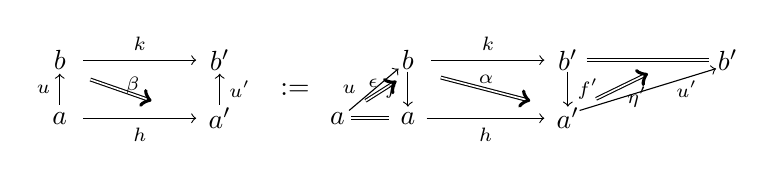
\begin{tikzpicture}[x=1.7em,y=1.4em]
  \node (bb)  at (0,1.5)  {$b$};
  \node (bbp) at (3.4,1.5) {$b'$};
  \node (ba)  at (0,0)    {$a$};
  \node (bap) at (3.4,0)  {$a'$};
  \draw[->] (0.5,1.5) -- node[above]{$\scriptstyle k$} (2.9,1.5);
  \draw[->] (0.5,0)   -- node[below]{$\scriptstyle h$} (2.9,0);
  \draw[->] (0,0.35)  -- node[left]{$\scriptstyle u$} (0,1.15);
  \draw[->] (3.4,0.35) -- node[right]{$\scriptstyle u'$} (3.4,1.15);
  \draw[->,double] (0.65,1.0) -- (1.95,0.45);
  \node[right] at (1.2,0.85) {$\scriptstyle\beta$};
  \node at (5.0,0.75) {$:=$};
  \node (qb)  at (7.4,1.5) {$b$};
  \node (qbp) at (10.8,1.5) {$b'$};
  \node (qbp2) at (14.2,1.5) {$b'$};
  \node (qa)  at (5.9,0) {$a$};
  \node (qam) at (7.4,0) {$a$};
  \node (qap) at (10.8,0) {$a'$};
  \draw[->] (7.9,1.5) -- node[above]{$\scriptstyle k$} (10.3,1.5);
  \draw[double] (11.2,1.5) -- (13.8,1.5);
  \draw[->] (6.15,0.2) -- (7.2,1.28);
  \node[left] at (6.5,0.75) {$\scriptstyle u$};
  \draw[->,double] (6.5,0.45) -- (7.15,0.95);
  \node[right] at (6.35,0.9) {$\scriptstyle\epsilon$};
  \draw[->] (7.4,1.2) -- node[left]{$\scriptstyle f$} (7.4,0.3);
  \draw[double] (6.2,0) -- (7.0,0);
  \draw[->] (7.8,0) -- node[below]{$\scriptstyle h$} (10.3,0);
  \draw[->,double] (8.1,1.05) -- (10.0,0.45);
  \node[right] at (8.7,1.0) {$\scriptstyle\alpha$};
  \draw[->] (10.8,1.2) -- node[right]{$\scriptstyle f'$} (10.8,0.3);
  \draw[->] (11.05,0.2) -- (13.95,1.28);
  \node[right] at (12.9,0.75) {$\scriptstyle u'$};
  \draw[->,double] (11.4,0.5) -- (12.5,1.15);
  \node[right] at (11.85,0.55) {$\scriptstyle\eta'$};
\end{tikzpicture}
\end{center}
\end{definition}

在该双射下相互对应的诸 2-\trCell{} \eqref{eq:mates-bijection} 称为%
\textbf{\trMate}（mates）。

\begin{example}\label{exa:conjugates}
这一\trMate{}可特殊化而定义一个双射：一边是介于一对平行的\trLeftAdjoint{}之间的%
2-\trCell，另一边是以相反方向介于它们的\trRightAdjoint{}之间的 2-\trCell——
Mac Lane 称之为\textbf{\trConjugate}（conjugates）\cite[\S IV.7]{bib81}：
\begin{center}
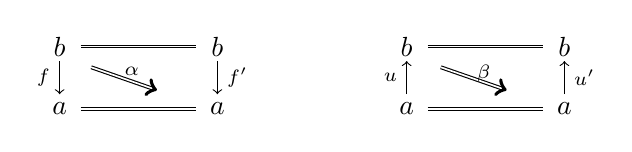
\begin{tikzpicture}[x=1.9em,y=1.5em]
  \node (cb) at (0,1.5)  {$b$};
  \node (cb2) at (3.0,1.5) {$b$};
  \node (ca) at (0,0)    {$a$};
  \node (ca2) at (3.0,0) {$a$};
  \draw[double] (0.4,1.5) -- (2.6,1.5);
  \draw[double] (0.4,0)   -- (2.6,0);
  \draw[->] (0,1.15)  -- node[left]{$\scriptstyle f$} (0,0.35);
  \draw[->] (3.0,1.15) -- node[right]{$\scriptstyle f'$} (3.0,0.35);
  \draw[->,double] (0.6,1.0) -- (1.85,0.45);
  \node[right] at (1.05,0.9) {$\scriptstyle\alpha$};
  \node at (4.8,0.75) {$\rightsquigarrow$};
  \node (db) at (6.6,1.5)  {$b$};
  \node (db2) at (9.6,1.5) {$b$};
  \node (da) at (6.6,0)    {$a$};
  \node (da2) at (9.6,0)   {$a$};
  \draw[double] (7.0,1.5) -- (9.2,1.5);
  \draw[double] (7.0,0)   -- (9.2,0);
  \draw[->] (6.6,0.35)  -- node[left]{$\scriptstyle u$} (6.6,1.15);
  \draw[->] (9.6,0.35)  -- node[right]{$\scriptstyle u'$} (9.6,1.15);
  \draw[->,double] (7.25,1.0) -- (8.5,0.45);
  \node[right] at (7.75,0.85) {$\scriptstyle\beta$};
\end{tikzpicture}
\end{center}
\end{example}

方块 \eqref{eq:mates-bijection} 的水平复合与竖直复合都保持这一\trMate，其确切
含义由如下结果阐明：

\begin{theorem}[\trMate{}的双函子性]\label{thm:mates-double-functoriality}
对任何 2-\trCategory，介于诸\trDoubleCategory{}之间存在一个双\trIsomorphism
$\mathbb{L}_{\mathrm{adj}}\cong\mathbb{R}_{\mathrm{adj}}$，这些\trDoubleCategory{}满足：
\begin{itemize}
\item 其对象与水平态射即诸对象与诸 1-\trCell；
\item 其竖直态射为完整指定的诸\trAdjunction{} $(f,u,\eta,\epsilon)$，指向%
\trLeftAdjoint{}的方向；\footnote{竖直态射的复合用到第 2 章中的%
\cref{prop:adjunctions-compose}的证明中给出的构造。}
\item $\mathbb{L}_{\mathrm{adj}}$ 中的胞腔是下方左侧所示形状的 2-\trCell，而
  $\mathbb{R}_{\mathrm{adj}}$ 中的胞腔是下方右侧所示形状的 2-\trCell：
\begin{center}
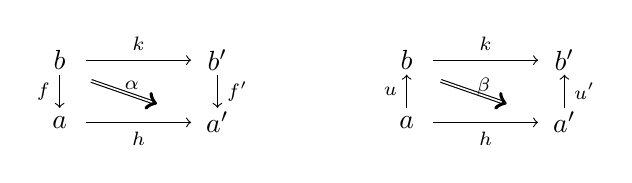
\begin{tikzpicture}[x=1.9em,y=1.5em]
  \node (eb) at (0,1.5) {$b$};
  \node (ebp) at (3.0,1.5) {$b'$};
  \node (ea) at (0,0) {$a$};
  \node (eap) at (3.0,0) {$a'$};
  \draw[->] (0.5,1.5) -- node[above]{$\scriptstyle k$} (2.5,1.5);
  \draw[->] (0.5,0)   -- node[below]{$\scriptstyle h$} (2.5,0);
  \draw[->] (0,1.15)  -- node[left]{$\scriptstyle f$} (0,0.35);
  \draw[->] (3.0,1.15) -- node[right]{$\scriptstyle f'$} (3.0,0.35);
  \draw[->,double] (0.6,1.0) -- (1.85,0.45);
  \node[right] at (1.05,0.9) {$\scriptstyle\alpha$};
  \node (fb) at (6.6,1.5) {$b$};
  \node (fbp) at (9.6,1.5) {$b'$};
  \node (fa) at (6.6,0) {$a$};
  \node (fap) at (9.6,0) {$a'$};
  \draw[->] (7.1,1.5) -- node[above]{$\scriptstyle k$} (9.1,1.5);
  \draw[->] (7.1,0)   -- node[below]{$\scriptstyle h$} (9.1,0);
  \draw[->] (6.6,0.35)  -- node[left]{$\scriptstyle u$} (6.6,1.15);
  \draw[->] (9.6,0.35)  -- node[right]{$\scriptstyle u'$} (9.6,1.15);
  \draw[->,double] (7.25,1.0) -- (8.5,0.45);
  \node[right] at (7.75,0.85) {$\scriptstyle\beta$};
\end{tikzpicture}
\end{center}
\end{itemize}
这一双\trIsomorphism{}在对象以及水平与竖直态射上充当恒等，而在胞腔上的作用
则是取\trMate。\footnote{\trDoubleCategory{}的这个双\trIsomorphism{}可视为定义了一个 2-自然%
\trIsomorphism{}的某个分量，而该 2-自然\trIsomorphism{}则介于 2-\trFunctor{}
$\mathbb{L}_{\mathrm{adj}}$、$\mathbb{R}_{\mathrm{adj}}\colon 2\text{-}\mathit{Cat}\to\mathsf{Dbl}\text{-}\mathit{Cat}$
之间——后者从 $2\text{-}\mathit{Cat}$ 映到由\trDoubleCategory、
双\trFunctor{}与水平\trNaturalTransformation{}组成的 2-\trCategory。}
\end{theorem}

\begin{proof}
这一\trMate{}的水平与竖直函子性可通过在\trPastingDiagram{}中追图来验证
（或参见 \cite[2.2]{bib70}）。
\end{proof}

\begin{warning}[同构的\trMate{}未必是同构]\label{war:mates-of-isomorphisms}
一般地说，\eqref{eq:mates-bijection} 的一对相互对应的 2-\trCell{}之中的某一个
可为\trInvertible{}而另一个不然。例如，\trAdjunction{} $f\dashv u$ 的\trUnit{}与%
\trCounit{}各自既可与恒等\trCell{} $\mathrm{id}_{f}$ 相对应、又可与恒等\trCell
$\mathrm{id}_{u}$ 相对应，视这些 2-\trCell{}以何种方式被安放进方块而定
（见\cref{ex:mates-identity-cells}）。然而，若两个水平 1-\trCell{} $h$ 与 $k$
都是\trEquivalence，或者两个\trAdjunction{} $f\dashv u$ 与 $f'\dashv u'$ 都是%
\trAdjointEquivalence，则 $\alpha\colon f'k\Rightarrow hf$ 是\trInvertible
当且仅当其\trMate{} $\beta\colon ku\Rightarrow u'h$ 是\trInvertible。
\end{warning}

在\cref{war:mates-of-isomorphisms}的基础上，我们有：

\begin{proposition}[伴随性的等价不变性]\label{prop:equivalence-invariance-of-adjointness}
设给定一个本质交换的方块，其水平箭头均为\trEquivalence：
\begin{center}
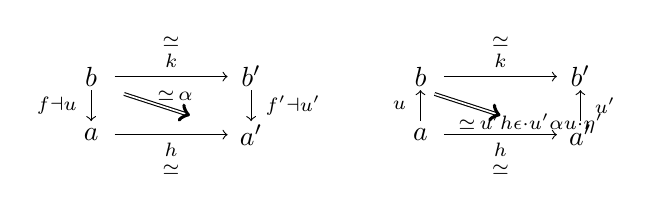
\begin{tikzpicture}[x=1.7em,y=1.4em]
  \node (gb) at (1.4,1.5) {$b$};
  \node (gbp) at (4.8,1.5) {$b'$};
  \node (ga) at (1.4,0) {$a$};
  \node (gap) at (4.8,0) {$a'$};
  \draw[->] (1.9,1.5) -- (4.3,1.5);
  \node at (3.1,1.9) {$\scriptstyle k$};
  \node at (3.1,2.4) {$\scriptstyle\simeq$};
  \draw[->] (1.9,0) -- (4.3,0);
  \node at (3.1,-0.4) {$\scriptstyle h$};
  \node at (3.1,-0.9) {$\scriptstyle\simeq$};
  \draw[->] (1.4,1.15) -- (1.4,0.35);
  \node[left] at (1.3,0.75) {$\scriptstyle f\dashv u$};
  \draw[->] (4.8,1.15) -- (4.8,0.35);
  \node[right] at (4.9,0.75) {$\scriptstyle f'\dashv u'$};
  \draw[->,double] (2.1,1.05) -- (3.5,0.5);
  \node[right] at (2.6,1.0) {$\scriptstyle\simeq\,\alpha$};
  \node at (6.6,0.75) {$\rightsquigarrow$};
  \node (hb) at (8.4,1.5) {$b$};
  \node (hbp) at (11.8,1.5) {$b'$};
  \node (ha) at (8.4,0) {$a$};
  \node (hap) at (11.8,0) {$a'$};
  \draw[->] (8.9,1.5) -- (11.3,1.5);
  \node at (10.1,1.9) {$\scriptstyle k$};
  \node at (10.1,2.4) {$\scriptstyle\simeq$};
  \draw[->] (8.9,0) -- (11.3,0);
  \node at (10.1,-0.4) {$\scriptstyle h$};
  \node at (10.1,-0.9) {$\scriptstyle\simeq$};
  \draw[->] (8.4,0.35) -- (8.4,1.15);
  \node[left] at (8.3,0.75) {$\scriptstyle u$};
  \draw[->] (11.8,0.35) -- (11.8,1.15);
  \node[right] at (11.9,0.75) {$\scriptstyle u'$};
  \draw[->,double] (8.7,1.05) -- (10.1,0.5);
  \node[right] at (9.0,0.28) {$\scriptstyle\simeq\,u'h\epsilon\cdot u'\alpha u\cdot\eta'$};
\end{tikzpicture}
\end{center}
则 $f$ 容许一个\trRightAdjoint{} $u$，当且仅当 $f'$ 容许一个\trRightAdjoint{}
$u'$；此时，同构 $\alpha$ 的\trMate{}是一个\trIsomorphism。
\end{proposition}

\begin{proof}
第 2 章中的\cref{prop:adjoint-equivalences}可用来选取互逆的\trAdjointEquivalence
$k'\dashv k$ 与 $h\dashv h'$。若 $f$ 是一个\trLeftAdjoint，则由第 2 章中的%
\cref{prop:adjunctions-compose}，$f'\cong hfk'$ 同构于一个\trLeftAdjoint，于是由
第 2 章中的\cref{prop:uniqueness-of-adjoints}，$f'$ 是 $kuh'$ 的\trLeftAdjoint。
$f'\dashv u'$ 被定义为如前一段所示的复合\trAdjunction，则 $\alpha$ 的\trMate{}算出来
是 $h'h\cong\mathrm{id}_{a}$ 与 $ku$ 的须状复合。由第 2 章中的%
\cref{prop:uniqueness-of-adjoints}，$f'$ 的\trRightAdjoint{}的任何其他选取都与
这一个同构，故 $\alpha$ 的\trMate{}仍是一个\trIsomorphism。
\end{proof}

\cref{ex:left-adjoints-isomorphic}提示了一个新证明：拥有公共右伴随的任意一对%
\trLeftAdjoint{} $f'\dashv u$ 与 $f\dashv u$ 都是同构的
（见第 2 章中的\cref{prop:uniqueness-of-adjoints}）——只需运用双%
\trIsomorphism{} $\mathbb{L}_{\mathrm{adj}}\cong\mathbb{R}_{\mathrm{adj}}$。
沿同一路线的一个更复杂的论证则可用来证明：

\begin{lemma}\label{lem:adjoint-triple-invertible-cells}
设给定\trFunctor{}的一个\trAdjointTriple{} $\ell\dashv i\dashv r$。则 $\ell\dashv i$
的\trCounit{}是\trInvertible，当且仅当 $i\dashv r$ 的\trUnit{}是\trInvertible。
\end{lemma}

\begin{proof}
设 $i\colon a\to b$，并记 $\epsilon\colon\ell i\Rightarrow\mathrm{id}_{a}$ 为
$\ell\dashv i$ 的\trCounit、$\eta\colon\mathrm{id}_{a}\Rightarrow ri$ 为
$i\dashv r$ 的\trUnit。若 $\epsilon$ 容许一个逆\trIsomorphism
$\epsilon^{-1}\colon\mathrm{id}_{a}\Rightarrow\ell i$%
\footnote{原书印作「$\epsilon^{-1}\colon\ell i\Rightarrow\mathrm{id}_{a}$」，
与 $\epsilon$ 同向。逆\trIsomorphism{}的方向应当相反，且本节下文总结处原书
亦自印作「$\epsilon^{-1}\colon\mathrm{id}_{a}\Rightarrow\ell i$」，疑为笔误，
此处径改。——译者注}，则下方左侧所示的 $\mathbb{L}_{\mathrm{adj}}$ 中的竖直
复合，容许下方右侧所示的胞腔作为其关于水平复合的逆：
\begin{center}
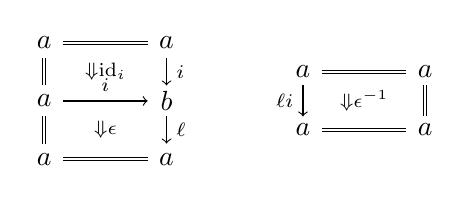
\begin{tikzpicture}[x=1.7em,y=1.4em]
  \node (m1) at (0,3) {$a$};
  \node (m2) at (2.6,3) {$a$};
  \draw[double] (0.4,3) -- (2.2,3);
  \draw[double] (0,2.6) -- (0,1.9);
  \draw[->] (2.6,2.6) -- node[right]{$\scriptstyle i$} (2.6,1.9);
  \node at (1.3,2.25) {$\scriptstyle\Downarrow\mathrm{id}_{i}$};
  \node (m3) at (0,1.5) {$a$};
  \node (m4) at (2.6,1.5) {$b$};
  \draw[->] (0.4,1.5) -- node[above]{$\scriptstyle i$} (2.2,1.5);
  \draw[double] (0,1.1) -- (0,0.4);
  \draw[->] (2.6,1.1) -- node[right]{$\scriptstyle\ell$} (2.6,0.4);
  \node at (1.3,0.75) {$\scriptstyle\Downarrow\epsilon$};
  \node (m5) at (0,0) {$a$};
  \node (m6) at (2.6,0) {$a$};
  \draw[double] (0.4,0) -- (2.2,0);
  \node (n1) at (5.5,2.25) {$a$};
  \node (n2) at (8.1,2.25) {$a$};
  \draw[double] (5.9,2.25) -- (7.7,2.25);
  \draw[->] (5.5,1.9) -- node[left]{$\scriptstyle\ell i$} (5.5,1.1);
  \draw[double] (8.1,1.9) -- (8.1,1.1);
  \node at (6.8,1.5) {$\scriptstyle\Downarrow\epsilon^{-1}$};
  \node (n3) at (5.5,0.75) {$a$};
  \node (n4) at (8.1,0.75) {$a$};
  \draw[double] (5.9,0.75) -- (7.7,0.75);
\end{tikzpicture}
\end{center}
运用双\trIsomorphism{} $\mathbb{L}_{\mathrm{adj}}\cong\mathbb{R}_{\mathrm{adj}}$
的水平函子性，这些胞腔的诸\trMate{}在 $\mathbb{R}_{\mathrm{adj}}$ 中水平复合亦必成为
恒等。\footnote{由于所论胞腔中的水平态射皆为恒等，\cref{war:mates-of-isomorphisms}中提出的顾虑在此并不适用。}运用双%
\trIsomorphism{} $\mathbb{L}_{\mathrm{adj}}\cong\mathbb{R}_{\mathrm{adj}}$ 的
竖直函子性，该竖直复合的\trMate{}等于 $\mathbb{R}_{\mathrm{adj}}$ 中的如下复合：
\begin{center}
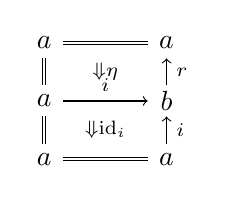
\begin{tikzpicture}[x=1.7em,y=1.4em]
  \node (o1) at (0,3) {$a$};
  \node (o2) at (2.6,3) {$a$};
  \draw[double] (0.4,3) -- (2.2,3);
  \draw[double] (0,2.6) -- (0,1.9);
  \draw[->] (2.6,1.9) -- node[right]{$\scriptstyle r$} (2.6,2.6);
  \node at (1.3,2.25) {$\scriptstyle\Downarrow\eta$};
  \node (o3) at (0,1.5) {$a$};
  \node (o4) at (2.6,1.5) {$b$};
  \draw[->] (0.4,1.5) -- node[above]{$\scriptstyle i$} (2.2,1.5);
  \draw[double] (0,1.1) -- (0,0.4);
  \draw[->] (2.6,0.4) -- node[right]{$\scriptstyle i$} (2.6,1.1);
  \node at (1.3,0.75) {$\scriptstyle\Downarrow\mathrm{id}_{i}$};
  \node (o5) at (0,0) {$a$};
  \node (o6) at (2.6,0) {$a$};
  \draw[double] (0.4,0) -- (2.2,0);
\end{tikzpicture}
\end{center}
从而 $\epsilon^{-1}$ 的\trMate{}必给出 $\eta$ 的逆。总而言之，我们看到：$\ell\dashv i$
的\trCounit{}是一个\trIsomorphism，当且仅当 $i\dashv r$ 的\trUnit{}是一个%
\trIsomorphism；此时，其逆\trIsomorphism{}
$\eta^{-1}\colon ri\Rightarrow\mathrm{id}_{a}$
便是 $\epsilon^{-1}\colon\mathrm{id}_{a}\Rightarrow\ell i$
经由复合\trAdjunction{} $\ell i\dashv ri$ 而得的\trConjugate{}：
\begin{center}
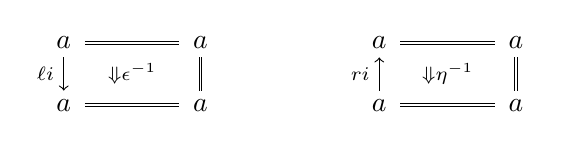
\begin{tikzpicture}[x=1.9em,y=1.5em]
  \node (p1) at (0,1.5) {$a$};
  \node (p2) at (2.6,1.5) {$a$};
  \draw[double] (0.4,1.5) -- (2.2,1.5);
  \draw[->] (0,1.15) -- node[left]{$\scriptstyle\ell i$} (0,0.35);
  \draw[double] (2.6,1.15) -- (2.6,0.35);
  \node at (1.3,0.75) {$\scriptstyle\Downarrow\epsilon^{-1}$};
  \node (p3) at (0,0) {$a$};
  \node (p4) at (2.6,0) {$a$};
  \draw[double] (0.4,0) -- (2.2,0);
  \node at (4.3,0.75) {$\rightsquigarrow$};
  \node (q1) at (6.0,1.5) {$a$};
  \node (q2) at (8.6,1.5) {$a$};
  \draw[double] (6.4,1.5) -- (8.2,1.5);
  \draw[->] (6.0,0.35) -- node[left]{$\scriptstyle ri$} (6.0,1.15);
  \draw[double] (8.6,1.15) -- (8.6,0.35);
  \node at (7.3,0.75) {$\scriptstyle\Downarrow\eta^{-1}$};
  \node (q3) at (6.0,0) {$a$};
  \node (q4) at (8.6,0) {$a$};
  \draw[double] (6.4,0) -- (8.2,0);
\end{tikzpicture}
\end{center}
\end{proof}

\subsection*{练习}

\begin{exercise}\label{ex:mates-identity-cells}
\begin{enumerate}[label=(\roman*)]
\item 说明 \eqref{eq:transposes} 的诸双射如何可以实现为\trMate{}的特殊情形。
\item 通过选取一对合适的\trAdjunction{}与\trFunctor，说明\trAdjunction{}
  $f\dashv u$ 的\trUnit{}如何与 $\mathrm{id}_{u}$ 相对应。
\item 通过选取一对合适的\trAdjunction{}与\trFunctor，说明\trAdjunction{}
  $f\dashv u$ 的\trUnit{}如何与 $\mathrm{id}_{f}$ 相对应。
\end{enumerate}
\end{exercise}

\begin{exercise}\label{ex:left-adjoints-isomorphic}
考虑 $\mathbb{L}_{\mathrm{adj}}\cong\mathbb{R}_{\mathrm{adj}}$ 中作为竖直态射的
一对\trAdjunction{} $f\dashv u$ 与 $f'\dashv u$，并运用\trMate{}的双函子性证明
$f\cong f'$。
\end{exercise}

\begin{exercise}\label{ex:horizontal-vertical-mates}
考虑 2-\trCell
\begin{center}
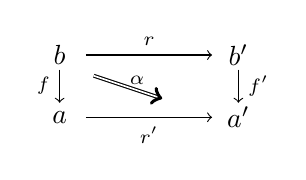
\begin{tikzpicture}[x=1.9em,y=1.5em]
  \node (wb)  at (0,1.5)  {$b$};
  \node (wbp) at (3.4,1.5) {$b'$};
  \node (wa)  at (0,0)    {$a$};
  \node (wap) at (3.4,0)  {$a'$};
  \draw[->] (0.5,1.5) -- node[above]{$\scriptstyle r$} (2.9,1.5);
  \draw[->] (0.5,0)   -- node[below]{$\scriptstyle r'$} (2.9,0);
  \draw[->] (0,1.15)  -- node[left]{$\scriptstyle f$} (0,0.35);
  \draw[->] (3.4,1.15) -- node[right]{$\scriptstyle f'$} (3.4,0.35);
  \draw[->,double] (0.65,1.0) -- (1.95,0.45);
  \node[right] at (1.15,0.9) {$\scriptstyle\alpha$};
\end{tikzpicture}
\end{center}
其中竖直 1-\trCell{}容许\trRightAdjoint{} $f\dashv u$ 与 $f'\dashv u'$，水平
1-\trCell{}容许\trLeftAdjoint{} $\ell\dashv r$ 与 $\ell'\dashv r'$。证明：$\alpha$
关于诸竖直\trAdjunction{}的\trMate{}定义一个\trIsomorphism{} $ru\cong u'r'$，当且仅当
$\alpha$ 关于诸水平\trAdjunction{}的\trMate{}定义一个\trIsomorphism{}
$\ell'f'\cong f\ell$——并且，就诸复合\trAdjunction{}而言，这两个\trIsomorphism{}%
本身即在\cref{exa:conjugates}的意义下相互对应。
\end{exercise}

\begin{exercise}\label{ex:two-functor-preserves-mates}
证明任何 2-\trFunctor{} $F\colon\mathcal{C}\to\mathcal{D}$ 都保持%
\trEquivalence、\trAdjunction{}与\trMate。
\end{exercise}

